%
% File emnlp2019.tex
%
%% Based on the style files for ACL 2019, which were
%% Based on the style files for EMNLP 2018, which were
%% Based on the style files for ACL 2018, which were
%% Based on the style files for ACL-2015, with some improvements
%%  taken from the NAACL-2016 style
%% Based on the style files for ACL-2014, which were, in turn,
%% based on ACL-2013, ACL-2012, ACL-2011, ACL-2010, ACL-IJCNLP-2009,
%% EACL-2009, IJCNLP-2008...
%% Based on the style files for EACL 2006 by 
%%e.agirre@ehu.es or Sergi.Balari@uab.es
%% and that of ACL 08 by Joakim Nivre and Noah Smith

\documentclass[11pt,a4paper]{article}
\usepackage[hyperref]{emnlp-ijcnlp-2019}
\usepackage{times}
\usepackage{latexsym}
\usepackage{graphicx}  %%% for including graphics
\usepackage{booktabs}
\usepackage{xspace}
\usepackage{multirow}
\usepackage{url}

%\aclfinalcopy % Uncomment this line for the final submission

%\setlength\titlebox{5cm}
% You can expand the titlebox if you need extra space
% to show all the authors. Please do not make the titlebox
% smaller than 5cm (the original size); we will check this
% in the camera-ready version and ask you to change it back.

\newcommand\BibTeX{B{\sc ib}\TeX}
\newcommand\confname{EMNLP-IJCNLP 2019}
\newcommand\conforg{SIGDAT}
\newcommand{\refexp}[1]{\textsl{#1}}
\newcommand{\word}[1]{\textsl{#1}}
\newcommand{\cat}[1]{\textsc{#1}}
\newcommand{\vgenome}{VisualGenome\xspace}
\newcommand{\ra}{$\rightarrow$}

\newcommand{\sz}[1]{\textcolor{blue}{\emph{//sz: #1//}}}
\newcommand{\gbt}[1]{\textcolor{orange}{\emph{//g: #1//}}}
\newcommand{\cs}[1]{\textcolor{green!60!black}{\emph{//cs: #1//}}}

\title{Supplemental Material for submission ``Do Objects in Real-World Images Have a Canonical Name?''}

\author{First Author \\
  Affiliation / Address line 1 \\
  Affiliation / Address line 2 \\
  Affiliation / Address line 3 \\
  {\tt email@domain} \\\And
  Second Author \\
  Affiliation / Address line 1 \\
  Affiliation / Address line 2 \\
  Affiliation / Address line 3 \\
  {\tt email@domain} \\}

\date{}

\begin{document}
\maketitle
\section{Dataset: Supplementary Information}
\label{app:instructions}

Figures~\ref{fig:instructions1} and~\ref{fig:instructions2} contain the instructions for our subjects in the first round and rounds 2-4, respectively.
After the first round, based on the opt-out annotation, we kept images that met all the following conditions (thresholds were estimated via manual inspection). This yielded $25,596$ images, discarding $5,497$.

\begin{itemize}
\item they were not marked as occluded by any subject;
\item ``Bounding box is unclear'' was marked at most twice;
\item at most 17\% of elicited names were in plural form (to remove cases where the bounding box contains several objects);
\item the most frequent elicited name is of the same domain as the \vgenome name.
\end{itemize}

Table~\ref{tab:overview_dataset2} gives an overview of the collection synsets, XXX, XXX, grouped into the $7$~domains.
\gbt{@Carina, the table doesn't fit, maybe put one domain x row?}

\begin{table*}[htb]
\small
	\begin{tabular}{@{~}l@{~}l@{~}l@{~}l@{~}l@{~}l@{~}l}
	\toprule
	        animals\_plants &               vehicles &                        home &                clothing &                   buildings &                    food &                 people \\
	\midrule
	  ungulate$_1$ (2037) &  aircraft$_1$ (1208) &  furnishing$_2$ (5355) &  shirt$_1$ (968) &  house$_1$ (364) &  dish$_2$ (812) &  woman$_1$ (1768) \\
	 horse$_1$ (833) &  train$_1$ (957) &  vessel$_3$ (525) &  overgarment$_1$ (786) &  bridge$_1$ (297) &  baked\_goods$_1$ (770) &  man$_1$ (1167) \\
	  feline$_1$ (763) &  car$_1$ (727) &  kitchen\_utensil$_1$ (132) &  dress$_1$ (199) &  shelter$_1$ (169) &  foodstuff$_2$ (280) &  male\_child$_1$ (853) \\
	 dog$_1$ (688) &  motorcycle$_1$ (564) &  crockery$_1$ (92) &  headdress$_1$ (135) &  restaurant$_1$ (58) &  vegetable$_1$ (48) &  athlete$_1$ (396) \\
	  bird$_1$ (389) &  truck$_1$ (559) &  cutlery$_2$ (82) &  neckwear$_1$ (65) &  outbuilding$_1$ (31) &  edible\_fruit$_1$ (42) &  child$_1$ (333) \\
	  flower$_1$ (44) &  boat$_1$ (499) &  tool$_1$ (72) &  robe$_1$ (27) &  hotel$_1$ (19) &  beverage$_1$ (23) &  creator$_2$ (11) \\
	  rodent$_1$ (27) &  ship$_1$ (38) &  lamp$_1$ (34) &  glove$_2$ (7) &  housing$_1$ (17) &   &  professional$_1$ (5) \\
	 insect$_1$ (12) &   &   &  footwear$_1$ (5) &  place\_of\_worship$_1$ (12) &   &   \\
	  fish$_1$ (11) &   &   &   &   &   &   \\
	\bottomrule
\end{tabular}
	\caption{Overview of our dataset: Synset nodes for each domain (subscript indicates synset number; number of instances in parentheses). \textbf{double-check} \label{tab:overview_dataset2}}
      \end{table*}
      
\begin{figure*}[htb]
  \centering
  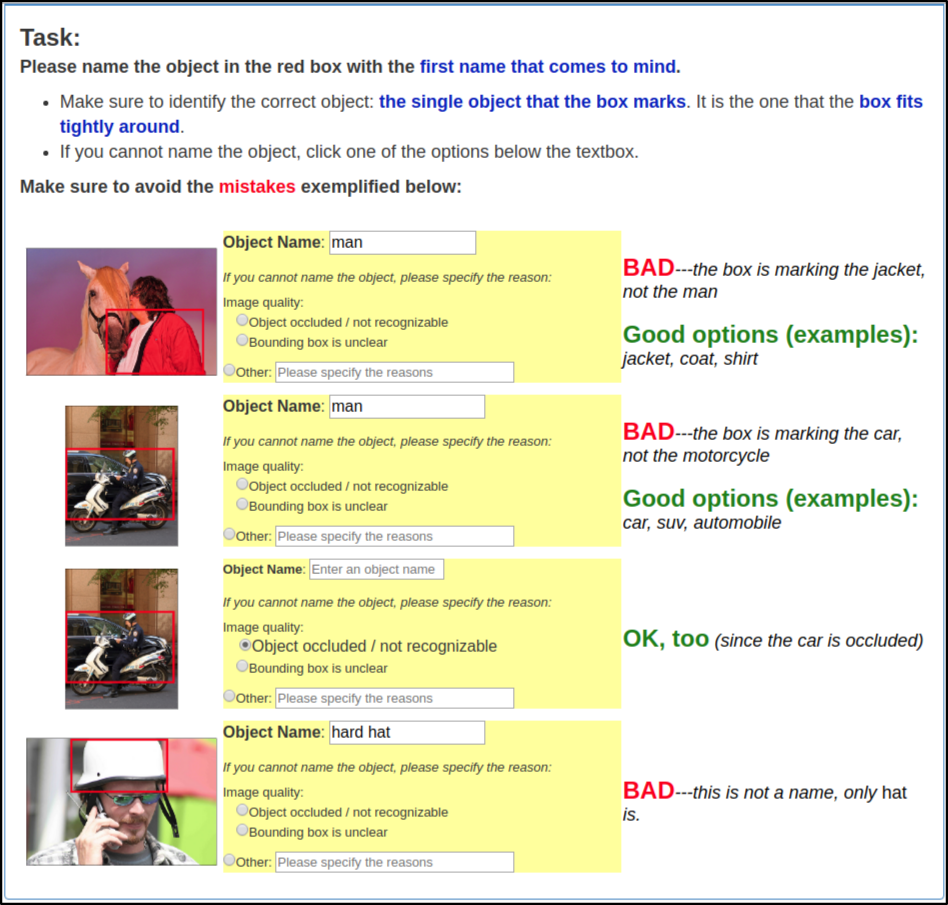
\includegraphics[width=1.5\columnwidth]{figures/round0.png}
  \caption{Instructions for AMT annotators for the first round.}
  \label{fig:instructions1}
\end{figure*}

\begin{figure*}[htb]
  \centering
  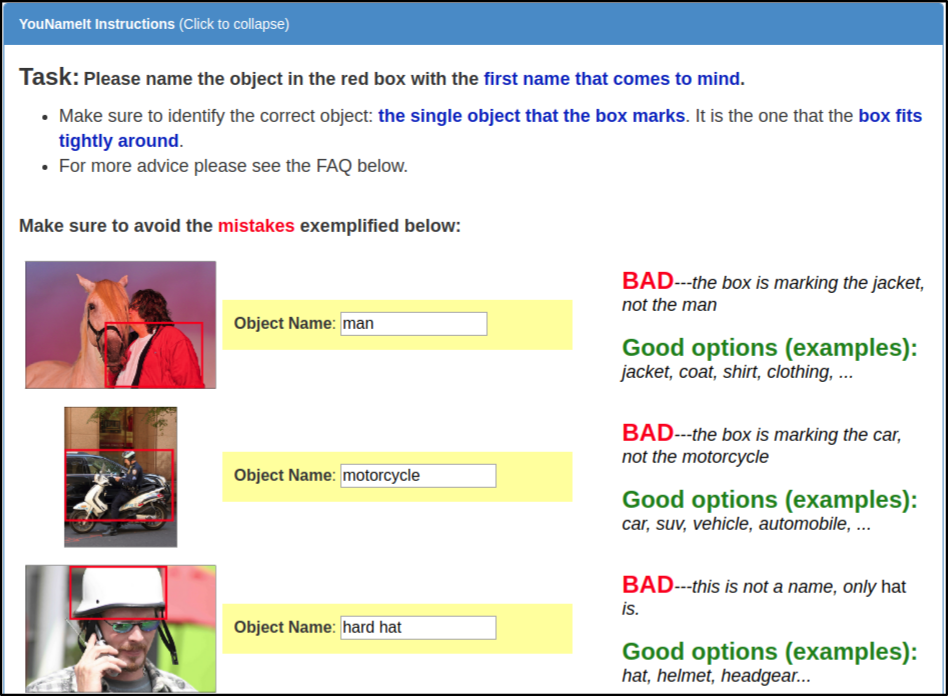
\includegraphics[width=1.5\columnwidth]{figures/round1+_p1.png}
  \caption{Instructions for AMT annotators for rounds~$2$ to~$4$. They were accompanied by the FAQ in Figure~\ref{fig:faq}}
  \label{fig:instructions2}
\end{figure*}

\begin{figure*}[htb]
  \centering
  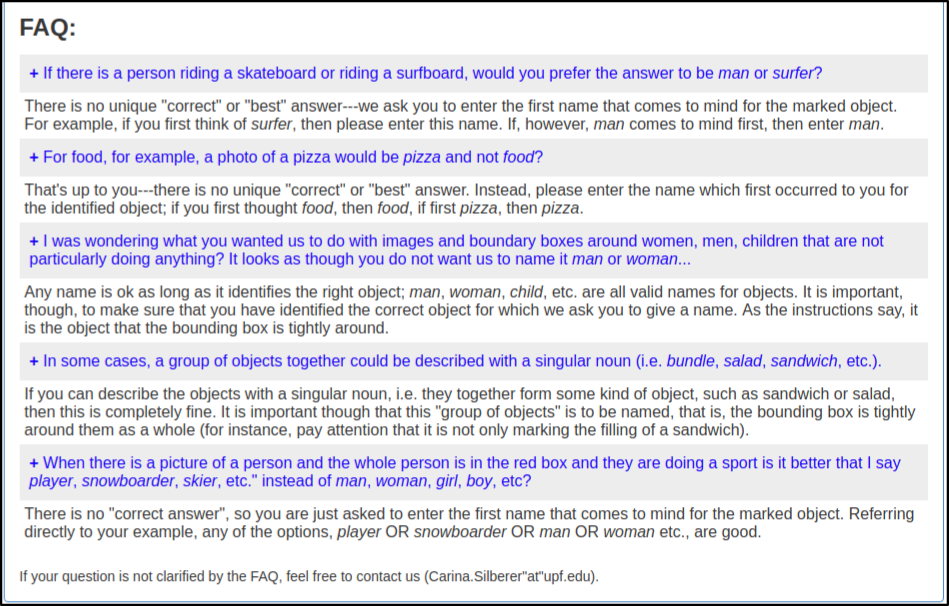
\includegraphics[width=1.5\columnwidth]{figures/round1+_p2.png}
  \caption{FAQ accompanying the instructions for AMT annotators for rounds~$2$ to~$4$.}
  \label{fig:faq}
\end{figure*}

\end{document}


%%% Local Variables:
%%% mode: latex
%%% TeX-master: t
%%% End:
